\documentclass[tikz,border=5mm]{standalone}
\usepackage{tkz-euclide}
\usetikzlibrary{calc,intersections}

\begin{document}
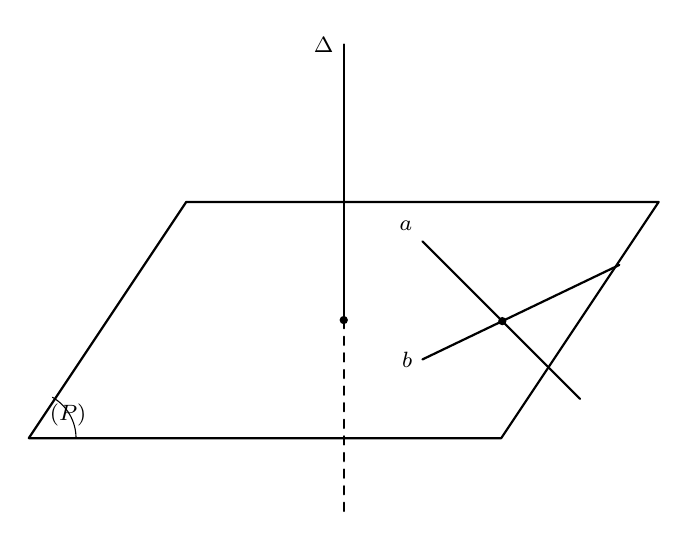
\begin{tikzpicture}[font=\footnotesize, line cap=round, line join=round, >=stealth]

% Định nghĩa các điểm của mặt phẳng (P) - Hình bình hành
\coordinate (A) at (0,0);
\coordinate (B) at (6,0);
\coordinate (C) at (8,3);
\coordinate (D) at (2,3);

% Vẽ mặt phẳng (P)
\draw[thick] (A) -- (B) -- (C) -- (D) -- cycle;

% Ký hiệu (P) ở góc
\node at (0.5, 0.3) {$(P)$};
\draw (A) ++(0.6,0) arc (0:60:0.6);

% Đường thẳng Delta (thẳng đứng)
\coordinate (T) at (4, 5);    % Điểm trên cao
\coordinate (I) at (4, 1.5);  % Giao điểm với mặt phẳng (nằm trong ABCD)
\coordinate (Bot) at (4, -1); % Điểm dưới thấp

% Vẽ phần Delta trên mặt phẳng (nhìn thấy)
\draw[thick] (T) node[left] {$\Delta$} -- (I);
\fill (I) circle (1.5pt); % Điểm giao cắt I

% Vẽ phần Delta dưới mặt phẳng (nét đứt)
\draw[dashed, thick] (I) -- (Bot);

% --- Vẽ hai đường thẳng a và b cắt nhau ---
% Định nghĩa tọa độ đầu cuối
\coordinate (a_start) at (5, 2.5);
\coordinate (a_end) at (7, 0.5);
\coordinate (b_start) at (5, 1);
\coordinate (b_end) at (7.5, 2.2);

% Vẽ đường a và đặt tên path
\draw[thick, name path=lineA] (a_start) node[above left] {$a$} -- (a_end);

% Vẽ đường b và đặt tên path
\draw[thick, name path=lineB] (b_start) node[left] {$b$} -- (b_end);

% Tìm giao điểm M của a và b
\path [name intersections={of=lineA and lineB, by=M}];
\fill (M) circle (1.5pt); % Vẽ giao điểm M

\end{tikzpicture}
\end{document}
